\chapter{General model equations for ICONAM}

\section{Introduction}

\footnote{This chaper copies in a wide part Gassmann and Herzog (2008).}When designing an atmospheric numerical model for the purpose of Numerical Weather Prediction (NWP) and climate simulations, a careful formulation of the continuous model equations is obviously the first step to be done. Closely connected, the construction of a physically adequate numerical scheme follows as the second step to form eventually a satisfactory discrete analogue. The paper deals with both of these main points. First, we start formulating a continuous model equation set, which is consistent with respect to energy, mass, and Ertel's (1942) potential vorticity (EPV) conservation. It is written in Poisson bracket form applying elements from N\'evir's (1998, 2004) atmospheric energy-vorticity-theory and also the Hamiltonian description from Morrison (1998) for an ideal fluid. Second, we are going to propose a method how to construct the discrete analogue of the Poisson brackets both in space and time. This philosophy allows us to retain the continuous conservation properties as already demonstrated impressively by Salmon (2004, 2005, 2007) concerning the spatial dicretisation.

From the point of view of theoretical meteorology the formulation of continuous model equations seems well established. Nevertheless, even today one becomes aware that notorious problems emerge when essaying to use in NWP in a consistent manner what is available from theory. In a recent paper Thuburn (2006) has carefully reviewed this dilemma how to design atmospheric models under the aspect of conservation properties.

In the present paper, we take up this problem for the compressible nonhydrostatic equations. This equation type became of common interest for modelling because of its suitability for atmospheric simulations over a wide range of meteorological phenomena from planetary down to local scales. Different nonhydrostatic regional models exist meanwhile as research and operational weather forecasting models.
Concerning global modelling, a notable development takes place in Japan (Satoh 2002, 2003), emphasizing  the careful inclusion of moist processes and conservative properties in the numerical scheme. Ultimately, this development is directed towards a global climate model with improved cloud-radiation interaction. A particular example of the application of compressible nonhydrostatic equations over the globe is the Unified Model of the UK Met Office (Davies et al.~2005) based on a thorough research work with a fairly general conception to use it as a global NWP-model, and for climate simulations as well. In our case we are motivated to deal with this model type in a running project to develop also a new global NWP and climate simulation model, called ICON (ICOsahedral Nonhydrostatic general circulation) model.

In the following approach we take advantage of our experience with the compressible nonhydrostatic Lokal-Modell (LM) (Doms and Sch\"attler 2002, Gassmann and Herzog 2007), which runs as a limited-area model operationally in the German Weather Service. The basic equations of the LM are on principle of rather general validity to use them also as a ground to formulate a global model. Our demanding approach begins with an equation set considering an atmosphere consisting of dry air and water vapour as gaseous components, with the addition of water in liquid and solid form (cloud drops, cloud ice, precipitating drops and ice particles). The conceptual way to take into account a multi-component system is borrowed from Wacker et al.~(2006). Additionally, the complete equation system is written by applying a mass-weighted turbulence averaging (known as Hesselberg averaging). With minute approximations this equation set serves us as a reference model, having mass-, energy- and EPV conservation.

Further, we introduce common approximations to arrive at realistic averaged model equations available in a more meteorological form with temperature and pressure as model variables. Molecular fluxes are neglected compared to the corresponding turbulent fluxes. In such a way, the model equations are equations of averaged quantities, where the molecular dissipation of kinetic energy is missed and should be replaced by turbulent dissipation as a remedy to obtain energy conserving model equations. The mass conservation is simply fulfilled and it is shown what mass control conditions for the partial mass budget equations of the multi-component system are necessary to be considered (Wacker et al., 2006). It is shown that the EPV is also a conservable quantity.
On this way, we have found a full-physics model equation set appropriate to apply the Hamiltonian tool. 
We invoke this theory, because to the best of our belief a Poisson bracket form with its specific antisymmetric property offers an interesting new way to find conservative numerical analogues (Salmon, 2004, 2005, 2007). We will show that it is possible to find a turbulence-averaged compressible nonhydrostatic model equation set in Poisson bracket form including all water constituents, precipitation fluxes, and diabatic sources/sinks in such a way that in the limit case for an ideal fluid the bracket form for a rotating atmosphere is exactly recovered. Hamiltonian theory for an ideal fluid is actually  applicable beyond this physical limitation. The bracket approach provides a compact functional evolution equation from which it is easy to derive corresponding model equation sets in a well-structured form using different reasonable model variables.

Salmon (2004, 2005, 2007) was inspired from the idea to retain the antisymmetry properties of dynamic brackets during model discretisation, in particular for the shallow-water equations, using the Poisson bracket formulation first, and then the more general Nambu bracket approach to construct conservative spatial schemes. Later on, we show a method how to formulate a numerical scheme both in space and time using the Poisson bracket form of the consistently derived nonhydrostatic compressible equations. Thereby, we closely follow Salmon's suggestions representing global integrals by global sums, and considering the rule of integration by parts in the spatial numerics. But here, the rule of integration by parts in the time scheme is also required, if one of the brackets occurs in different prognostic model equations.

\section{Reference equation set for a heterogeneous system}
As a first point, we think of a quite general compressible nonhydrostatic equation set describing a atmospheric  heterogeneous flow regime. Heterogeneity means here a two-component system consisting of dry air and water. Water is assumed to occur in all three phases including precipitating drops and ice particles. With reference to Wacker et al.~(2006) partial densities $\varrho_i$ are introduced and summed up to total density for this atmospheric mixture, $\varrho=\Sigma \varrho_i$, where the subscripts $i=d, v, l, f, r, p$ refer to dry air, water vapour, liquid and frozen cloud particles, rain drops and precipitating ice particles (snow, graupel etc.), respectively. A reference velocity vector is defined as a weighted mean, $\mathbf{v}= \Sigma \varrho_i \mathbf{v}_i / \varrho $. Due to this, an equation set for the mixture can be found, where the momentum equation, the continuity equation and the internal energy equation in this system is formed each as a sum from its separate component equations. We follow here the theoretical foundation of Wacker et al. (2006) who discuss the Cauchy form conservation of the momentum equation for a multicomponent system in their Section 3 with further supporting references as Gyarmati (1970) and Doms and Herbert (1985). Lange (2002) presents the same problem in his textbook. An alternative foundation is given by Bannon (2002) who considered a different reference velocity with respect to dry air. We do not pursue this way.
In a further procedure we carry out a turbulence (Reynolds-) averaging for these equations, where a barycentric mean (Hesselberg, 1925) with respect to the total density is used, $\hat{\psi}={\overline{\varrho \psi }}/{\bar{\varrho}}$, having $\psi = \hat{\psi}+ \psi^{''}$ for the considered variables. On this line we arrive at a sufficiently general equation set. It may read
\begin{align}
\bar{\varrho}\frac{\hat{d}\hat{\mathbf{v}}}{dt}
=&-\nabla\bar{p}-\bar{\varrho}\nabla\Phi
-2 \mathbf{\Omega}\times \bar{\varrho}\hat{\mathbf{v}}
+\nabla\cdot(\bar{\underline{\mathbf{F}}} - \overline{\varrho \mathbf{v}^{''}\mathbf{v}^{''}})\label{equ1}\\
\frac{\hat{d}\bar{\varrho}}{dt}
=& - \bar{\varrho}\nabla\cdot \hat{\mathbf{v}}\label{equ2}\\
\bar{\varrho}\frac{\hat{d}\hat{u}}{dt}
=&- \bar{p}\nabla\cdot \hat{\mathbf{v}} - \overline{p \nabla\cdot {\mathbf{v}}^{''}}
- \nabla\cdot( \overline{\mathbf{W}}+\overline{\varrho u^{''}\mathbf{v}^{''}})
+\bar{\underline{\mathbf{F}}}\cdot\cdot \nabla \hat{\mathbf{v}}
+\overline{\underline{\mathbf{F}}\cdot\cdot\nabla \mathbf{v}^{''}}\label{equ3}\\
\bar{\varrho}\frac{\hat{d}\hat{q}_{i}}{dt}
=&- \nabla\cdot( \overline{\mathbf{J}_{i}} + \overline{\varrho q_{i}^{''}\mathbf{v}^{''}}) + \bar{Q}_i .\label{equ4}
\end{align}
In order to spare writing the unaveraged multi-component equations originally assumed are easily obtained by omitting the turbulence averaging symbols and all the turbulence flux terms in the equations (1) - (4). The turbulence-averaged equations are the momentum equation (1), the continuity equation (2), the budget equation for the mean internal (heat) energy, $\hat{u}$, (3), and budget equations for the partial mass fractions, $\hat{q_i} =\bar{\varrho_i} / \bar{\varrho} $, (4), having $\Sigma \hat{q_i}=1 $. It is important to note that as a mass control condition the sum of the $\hat{q_i}$-budget equations over all $i$ have to yield the continuity equation (2), which implies $ \Sigma \overline{Q}_i=0$ ($\overline{Q}_d=0$) , $\Sigma \overline{\mathbf{J}}_{i}= 0 $ , $ \Sigma \overline{\varrho q_{i}^{''}\mathbf{v}^{''}}=0 $. Further explanations of symbols and terms in these equations are given in Table \ref{symbol_table}. In equation (3) and so in following
equations the notation $\cdot\cdot$ means the double scalar product between tensors. 
\begin{table}
\caption{Explanation of symbols.}
\centering
\begin{tabular}{|l|l|}
\hline
Symbol & Explanation \\
\hline
$\mathbf{v}_i$        &      velocity of i-th constituent  \\
${\mathbf{v}_i}^{(d)}:=\mathbf{v}_i - \mathbf{v}$ & diffusion velocity of  i-th constituent\\
$\mathbf{\Omega}$ & angular velocity of the Earth\\
$\Phi$ & geopotential\\
$Q_i$ &  source/sink-terms\\
$\mathbf{J}_{i}=\varrho_i {\mathbf{v}_i}^{(d)} $ & diffusion flux of i-th constituent\\
$\underline{\mathbf{F}}$ & viscous friction tensor\\
$\mathbf{J}_u$ & heat diffusion flux vector\\
$\mathbf{R}$ & radiation flux vector\\
$\mathbf{W}=\mathbf{J}_u + \mathbf{R}$ & composed heat flux vector\\
$\overline{\varrho \mathbf{v}^{''}\mathbf{v}^{''}}$ & turbulent momentum flux tensor\\
$\overline{\varrho u^{''}\mathbf{v}^{''}}$ & turbulent heat flux vector\\
$\overline{\varrho q_{i}^{''}\mathbf{v}^{''}}$ & turbulent vector flux of i-th partial \\ & mass fraction \\
$ \frac{\hat{d}}{dt}= \frac{\partial}{ \partial t} + \hat{\mathbf{v}} \cdot \nabla $
& av.~individual time change operator\\
\hline
\end{tabular}
\label{symbol_table}
\end{table}
Such atmospheric model equations do not govern, but rather attempt to represent real processes in the atmosphere. Such forms will never be exact, and approximations are unavoidable. These approximations must not violate the most important conservation properties regarding mass, energy and EPV. This should be a guide, when we are going to introduce further simplifications towards more practical model equations compared to the reference equation set. Our model equations are to be valid for turbulence-averaged variables with reference to (\ref{equ1})-(\ref{equ4}). This is an adequate assumption in view of realistic modelling accompanied by discretisations in space and time, where the turbulent flux terms represent subgrid scale processes determined by parameterisations.  We omit now as usual the viscous friction tensor against the turbulent momentum flux tensor, $-\overline{\varrho \mathbf{v}^{''} \mathbf{v}^{''}}\gg \overline{\underline{\mathbf{F}}}$, and so the molecular heat flux against the turbulent heat flux, $\overline{\varrho u^{''}\mathbf{v}^{''}}\gg \mathbf{J}_u$, from which we also have $\overline{\mathbf{W}}\Rightarrow \overline{\mathbf{R}}$. In the $\hat{q}_{i}$-budget equations (\ref{equ4}), however, the diffusion fluxes $\overline{\mathbf{J}}_{i}$ must not be dropped against the turbulent fluxes $\overline{\varrho q_{i}^{''}\mathbf{v}^{''}}$ in view of significant sedimentation (precipitation) fluxes. From energetical reasoning it is acceptable to neglect in the heat energy equation (\ref{equ3}) the direct energy transformation from mean kinetic energy to mean internal energy compared to the molecular dissipation term, $\overline{\underline{\mathbf{F}}\cdot\cdot\nabla \mathbf{v}^{''}} \gg \underline{\overline{\mathbf{F}}}\cdot\cdot\nabla\hat{\mathbf{v}}$.

With this approximations the averaged equation system becomes
\begin{align}
\bar{\varrho}\frac{\hat{d}\hat{\mathbf{v}}}{dt}
=&-\nabla\bar{p}-\bar{\varrho}\nabla\Phi
-2 \mathbf{\Omega}\times \bar{\varrho}\hat{\mathbf{v}}
+\nabla\cdot(- \overline{\varrho \mathbf{v}^{''}\mathbf{v}^{''}})
\label{equ5}\\
\frac{\hat{d}\bar{\varrho}}{dt}
= &- \bar{\varrho}\nabla\cdot \hat{\mathbf{v}}\label{equ6}\\
\bar{\varrho}\frac{\hat{d}\hat{u}}{dt}
=&- \nabla\cdot( \overline{\mathbf{R}}+\overline{\varrho u^{''}\mathbf{v}^{''}}) -\bar{p}\nabla\cdot \hat{\mathbf{v}} - \overline{p \nabla\cdot {\mathbf{v}}^{''}}
+\overline{\underline{\mathbf{F}}\cdot\cdot\nabla \mathbf{v}^{''}}\label{equ7}\\
\bar{\varrho}\frac{\hat{d}\hat{q}_{i}}{dt}
=&- \nabla\cdot( \overline{\mathbf{J}_{i}} + \overline{\varrho q_{i}^{''}\mathbf{v}^{''}}) + \bar{Q}_i .\label{equ8}
\end{align}
From the internal energy budget equation (\ref{equ7}) and a mechanical energy budget equation immediately derived from the momentum equation (\ref{equ5}),
\begin{equation}
\bar{\varrho}\frac{\hat{d}\left( \hat{\mathbf{v}}^2/2 + \Phi\right)}{dt} =-\nabla \cdot (  \bar{p}\hat{\mathbf{v}}-(- \overline{\varrho \mathbf{v}^{''}\mathbf{v}^{''}}) \cdot \hat{\mathbf{v}} ) + \bar{p} \nabla \cdot\hat{\mathbf{v}}
- (-\overline{\varrho \mathbf{v}^{''}\mathbf{v}^{''}}) \cdot \cdot \nabla\hat{\mathbf{v}} ,\label{equ9}
\end{equation}
a consistency requirement for the conservation of total energy budget as the sum of (\ref{equ7}) and (\ref{equ9}) can be inferred. Obviously, it reads
\begin{equation}
(-\overline{\varrho \mathbf{v}^{''}\mathbf{v}^{''}}) \cdot \cdot \nabla\hat{\mathbf{v}} + \overline{p \nabla\cdot {\mathbf{v}}^{''}} - 
\overline{\underline{\mathbf{F}}\cdot\cdot\nabla \mathbf{v}^{''}}=0 .
\label{equ10}
\end{equation} 
This requirement (\ref{equ10}) can be interpreted as the equilibrium case of a rudimentary mean turbulent kinetic energy equation formed from three terms which are shear production, buoyancy production and molecular dissipation.
With this reasoning we arrive eventually at an energy-consistent equation set,
using the abbreviation $\varepsilon = - \overline{\varrho \mathbf{v}^{''}\mathbf{v}^{''}}\cdot \cdot \nabla\hat{\mathbf{v}}> 0$ ,
\begin{align}
\bar{\varrho}\frac{\hat{d}\hat{\mathbf{v}}}{dt}=&-\nabla\bar{p}-\bar{\varrho}\nabla\Phi -2\mathbf{\Omega}\times\bar{\varrho}\hat{\mathbf{v}}-\nabla\cdot
\overline{\varrho \mathbf{v}^{''}\mathbf{v}^{''}}
\label{equ11}\\
\frac{\hat{d}\bar{\varrho}}{dt}=& -\bar{\varrho} \nabla\cdot \hat{\mathbf{v}} \label{equ12}\\
\bar{\varrho}\frac{\hat{d}\hat{u}}{dt}=& -\bar{p} \nabla\cdot \hat{\mathbf{v}}
-\nabla\cdot( \overline{\mathbf{R}}+\overline{\varrho u^{''}\mathbf{v}^{''}})
+ \varepsilon \label{equ13}\\
\bar{\varrho}\frac{\hat{d}\hat{q}_{i}}{dt}=&
-\nabla\cdot( \overline{\mathbf{J}_i} + \overline{\varrho q_{i}^{''}\mathbf{v}^{''}}) + \overline{Q_{i}}\;,
\label{equ14}
\end{align} 
together with a closed total energy budget
\begin{displaymath}
\bar{\varrho}\frac{\hat{d}\!\left( \hat{\mathbf{v}}^2\!/2\!+\! \Phi \!+ \!\hat{u}\right)}{dt} =-\!\nabla \!\cdot\!(  \bar{p}\hat{\mathbf{v}}+ \overline{\varrho \mathbf{v}^{''}\mathbf{v}^{''}} \!\cdot\! \hat{\mathbf{v}}+\overline{\mathbf{R}}+\overline{\varrho u^{''}\mathbf{v}^{''}}).
\end{displaymath}
In addition to this, we formulate also the budget equation for the EPV from the present system using (\ref{equ11}) and  (\ref{equ12}) with known operations. It follows
\begin{equation}
\bar{\varrho}\frac{\hat{d}}{dt}\left( \frac{\hat{\boldsymbol{\omega}}_a\cdot \nabla \hat{\psi} }{\bar{\varrho}}\right)=
-\nabla \cdot \left[\hat{\psi}\left(\nabla \frac{1}{\bar{\varrho}}\times\nabla
\bar{p}\right)-\hat{\boldsymbol{\omega}}_a \frac{\hat{d}\hat{\psi }}{d t}-\hat{\psi }
\left(\nabla \times \vec{\mathsf{R}} \right)\right].\label{equ16}
\end{equation}
For the vector $\vec{\mathsf{R}}$ we have
\begin{equation}
\vec{\mathsf{R}}=-\frac{\overline{\boldsymbol{\omega}^{''}\times \varrho \mathbf{v}^{''}}}{\bar{\varrho}}-\frac{1}{\bar{\varrho}}\overline{\varrho \nabla \frac{\mathbf{v}^{'' 2}}{2}} = -\frac{1}{\bar{\varrho}}
\nabla \cdot \overline{ \varrho \mathbf{v}^{''}\mathbf{v}^{''} },\label{equ17}
\end{equation} 
and, furthermore, $\hat{\psi}$ is an arbitrary scalar turbulence-averaged function, $\hat{\boldsymbol{\omega}}_a= \hat{\boldsymbol{\omega}}+2 \mathbf{\Omega}= \nabla\times \hat{\mathbf{v}}+2\mathbf{\Omega}$ is the mean absolute vorticity vector, and $\boldsymbol{\omega}^{''}= \nabla\times\mathbf{v}^{''} $ is the turbulent vorticity vector. As can be seen, the EPV is also a conservative quantity. It connects the vorticity nature of the turbulent flow with the total mass conservation and the moist thermodynamics (replacing $\hat{\psi}$ by a model-specific thermodynamic quantity which is still left open here).

\section{ Towards model equations applicable to a Poisson bracket form }
In the following we are interested in a more meteorological form of the equation set (\ref{equ11})-(\ref{equ14}) aiming at the model variables $\hat{\mathbf{v}},\hat{T},\bar{p},\hat{q_i}$ instead of $\hat{\mathbf{v}},\bar{\varrho},\hat{u},\hat{q_i}$. For that purpose the turbulence-averaged specific enthalpy $\hat{h}$ is introduced due to its relation to pressure and specific internal energy,
\begin{equation}
\overline{\varrho} \hat{h}= \overline{\varrho} \hat{u} + \overline{p} .\label{equ18}
\end{equation} 
Here, we make use of the assumption that the equation of state and so the nonlinear relation for the total specific enthalpy (\ref{equ21}) are valid for averaged quantities as an analogue to the unaveraged relations (cf. Herbert, 1975; Doms and Herbert, 1985)
\begin{equation}
\overline{p}=R_d \,\overline{\varrho} \,\hat{T}\, (1 + \hat{\alpha})  .\label{equ19}
\end{equation} 
$\hat{\alpha}$ means the averaged virtual increment,
\begin{equation}
\hat{\alpha} = \left( \frac{R_v}{R_d} - 1\right)\hat{q_v} - \hat{q_l} -
\hat{q_f} - \hat{q_r} - \hat{q_p} \label{equ20}
\end{equation} 
In a similar manner we yield for the nonlinear relation of the total specific enthalpy of the assumed mixture
\begin{equation}
\hat{h} = \Sigma \hat{h}_i \hat{q}_i , \label{equ21}
\end{equation} 
with 
\begin{equation}
\hat{h}_i = h_{0 i} + c_{p i} ( \hat{T} - T_0) \label{equ22}
\end{equation} 
for the specific enthalpy of the i-th component, and for the specific heat capacities we have 
\begin{equation}
\hat{c}_p = \Sigma c_{p i} \hat{q}_i \quad;\quad \hat{c}_v = \Sigma c_{v i} \hat{q}_i . \label{equ23}
\end{equation}  
By use of (\ref{equ18}) - (\ref{equ23}) we arrive after a straightforward analysis from  (\ref{equ13}) and (\ref{equ12}) at the desired prognostic equations for $\hat{T}$ and $\overline{p}$. This so-called meteorological form of the consistent equation set reads
\begin{align}
\bar{\varrho}\frac{\hat{d}\hat{\mathbf{v}}}{dt}=&-\nabla\bar{p}-
\bar{\varrho}\nabla\Phi -2\mathbf{\Omega}\times\bar{\varrho}\hat{\mathbf{v}}-\nabla\cdot \overline{\varrho \mathbf{v}^{''}\mathbf{v}^{''}}
\label{equ24}\\
\hat{c}_v \bar{\varrho}\frac{\hat{d}\hat{T}}{dt}=&-\bar{p} \nabla\cdot \hat{\mathbf{v}} + \bar{Q}_h + \bar{Q}_m \label{equ25}\\
\frac{\hat{d}\bar{p}}{dt}=&-\frac{\hat{c}_p }{\hat{c}_v }\bar{p} \nabla\cdot \hat{\mathbf{v}}+\left( \frac{\hat{c}_p}{\hat{c}_v } - 1 \right)  \bar{Q}_h  +\frac{\hat{c}_p}{\hat{c}_v }\bar{Q}_m \label{equ26}\\
\bar{\varrho}\frac{\hat{d}\hat{q}_{i}}{dt}=&-\nabla\cdot( \overline{\mathbf{J}_i} + \overline{\varrho q_{i}^{''}\mathbf{v}^{''}}) + \bar{Q}_i  \label{equ27}\\
\bar{p}=& R_d \bar{\varrho}\hat{T}( 1 + \hat{\alpha}).\label{equ28}
\end{align} 
The thermal source function $\bar{Q}_h$ and the moisture source function $\bar{Q}_m$ are defined as follows
\begin{align}
\bar{Q}_h =& - \nabla \cdot ( \overline{\mathbf{R}}+\overline{\varrho u^{''}\mathbf{v}^{''}}) - \Sigma{\hat{h}_i} \bar{\varrho} \frac{\hat{d}\hat{q_i}}{d t} + \varepsilon \label{equ29}\\
\bar{Q}_m =& R_d\hat{T} \bar{\varrho} \frac{\hat{d}\hat{\alpha}}{d t} .\label{equ30}
\end{align}

The derivation of the equation system (\ref{equ24})-(\ref{equ30}) needs, however, some more attention concerning mass conservation when sedimentation fluxes are incorporated in the water budget equations (\ref{equ27}). Invoking the approach of Wacker et al. (2006) (see also Catry et al. 2007), mass control conditions are necessary to be taken into account. One of them, $\Sigma \bar{\mathbf{J}_i} = 0$, is here of particular interest. Assuming diffusion fluxes given only in vertical direction, the precipitation fluxes (rain, snow etc.) are to be described by a common ansatz from Rogers and Yau (1989), $\bar{S_j}=-\bar{\mathbf{J}_j}=\bar{\varrho}\hat{q_j}\hat{V_j}^T$ for $j=r,p$ , where $\hat{V_j}^T$ is a terminal fall velocity to be parameterised. In order not to violate mass conservation it is important to consider the rest of diffusion fluxes, too, which have to play a compensating role. In the most simple way, these compensating fluxes may be read $\bar{J_i}=\bar{\varrho}\hat{q_i}\hat{w}^{(d)}$ for $i=d,v,l,f$ , assuming the same vertical diffusion velocity $\hat{w}^{(d)}$ instead of different $\hat{w_i}^{(d)}$. Thus we have
\begin{displaymath}
\hat{w}^{(d)} = \frac{\hat{q_r} \hat{V_r}^T+\hat{q_p} \hat{V_p}^T}{1 - \hat{q_r} - \hat{q_p}} \quad ,\label{equ31}
\end{displaymath}
and the $\hat{q_i}$ - budget equations (\ref{equ27}) read more specific
\begin{align}
\bar{\varrho}\frac{\hat{d}\hat{q}_{i}}{dt}&=
-\nabla\cdot \overline{\varrho q_{i}^{''}\mathbf{v}^{''}} - \frac{\partial\bar{\varrho}\hat{q_i}\hat{w}^{(d)}}{\partial z} + \bar{Q_{i}} \:;\:\:  i=d,v,l,f  \nonumber\\
\bar{\varrho}\frac{\hat{d}\hat{q}_{j}}{dt}&=
-\nabla\cdot \overline{\varrho q_{j}^{''}\mathbf{v}^{''}} + \frac{\partial\bar{\varrho}\hat{q_j}\hat{V_j}^T}{\partial z} + \bar{Q_{j}} \:;\:\:
 j=r, p \nonumber
\end{align}
The other mass control conditions are $\Sigma \hat{q_i} = 1$, $\Sigma \overline{\varrho q_{i}^{''}\mathbf{v}^{''}} = 0$, and $\Sigma \bar{Q_{i}} = 0$ with $\bar{Q_{d}}= 0$. 

In a further step the 'meteorological' system (\ref{equ24})-(\ref{equ30}) is now transformed into an obliging form in view of a Poisson bracket construction on the base of these equations. The works of Morrison (1998) and of N\'evir (1998) serve us as an example for the following analysis, though both authors have treated an ideal fluid compared to our much more realistic equation set. The treatment of N\'evir is from the meteorological point of view more interesting, because he includes the Coriolis effects, while Morrison has discussed a nonrotating system.  For the following we switch to the Eulerian form of our equation set, and we take into account density $\bar{\varrho}$ and virtual potential temperature $\hat{\theta_v}$  as prognostic variables instead of $\hat{T}$ and $\bar{p}$ in the previous set\footnote{The reason why we have chosen $\hat{\theta_v}$ is to arrive in (\ref{equ35}) at a tractable form of the pressure gradient term, and so to obtain simple functional derivatives in (\ref{equ46}) for the envisaged construction of a Poisson bracket form.}.
An important point is here the formulation of the momentum equation, where the advection term is identically reformulated due to the so-called Lamb transformation,
\begin{equation}
\mathbf{v} \cdot \nabla \mathbf{v} = \boldsymbol{\omega} \times \mathbf{v} + \nabla ( \frac{1}{2}\mathbf{v}^2 ) .\label{equ34}
\end{equation} 
We have decided to split off the advection term into a rotational term plus gradient of kinetic energy in order to unveil the ubiquitous vorticity process due to the rotational term, which otherwise would remain hidden. It is convenient to incorporate the Coriolis terms into one rotational term. In this point we follow the philosophy of N\'evir (1998). Moreover, the equation set is to be formulated in such a manner that in the limit case the equations for an ideal fluid are exactly recovered. The equation system equivalent to (\ref{equ24})-(\ref{equ30}) may be written in the following form
\begin{align}
\frac{\partial \hat{\mathbf{v}}}{\partial t} =& - \hat{\boldsymbol{\omega}}_a \times \hat{\mathbf{v}} - \nabla ( \frac{1}{2}\hat{\mathbf{v}}^2 + \Phi )
-\hat{\theta}_v \nabla (c_{pd}\bar{\Pi}) +  \vec{\mathsf{R}} \label{equ35} \\
\frac{\partial \bar{\varrho}}{\partial t} =& - \nabla \cdot ( \bar{\varrho} \hat{\mathbf{v}} )\label{equ36} \\
\frac{\partial (\bar{\varrho}\hat{\theta_v})}{\partial t} =& -\nabla \cdot ( \hat{\theta_v}\bar{\varrho} \hat{\mathbf{v}} )+ \bar{\varrho}\mathsf{Q}^{\left( \theta_v\right) }\label{equ37}\\
\frac{\partial ( \bar{\varrho} \hat{q}_i) }{\partial t} =& - \nabla \cdot( \bar{\varrho} \hat{q}_i \hat{\mathbf{v}} + \bar{\mathbf{J}}_i + \overline{\varrho q_i^{''}\mathbf{v}^{''}}) + \bar{Q}_i \label{equ38}\\
\bar{p} =& R_d\bar{\varrho} \hat{T}_v \label{equ39}\\
\hat{\theta}_v =& \hat{T}_v \left( \frac{p_{00}}{\bar{p}}\right)^{\frac{R_d}{c_{pd}}}=\frac{\hat{T}_v }{\bar{\Pi}}. \label{equ40}
\end{align}
$\bar{\Pi}$ is the Exner function as usual.
The source function $\mathsf{Q}^{\left(\theta_v\right)}$ in the $\hat{\theta}_v$-equation (\ref{equ37}) is defined by 
\begin{eqnarray}
c_{pd}\bar{\Pi}\,\bar{\varrho}\,\mathsf{Q}^{\left( \theta_v\right)}&=&
  \left( 1 + \frac{c_{pd}(1+\hat{\alpha})-\hat{c}_p}{\hat{c}_v}\right)  \bar{Q}_h\nonumber\\
&&+ \left( \frac{c_{pd}}{R_d} + \frac{c_{pd}(1+\hat{\alpha})-\hat{c}_p}{\hat{c}_v}\right)\bar{Q}_m  \nonumber\\
&&+ \left(\frac{c_{pd}(1+\hat{\alpha})-\hat{c}_p}{\hat{c}_v} \right) \left(- \bar{p} \nabla \cdot \hat{\mathbf{v}} \right).\label{equ42}
\end{eqnarray}
Strictly speaking, $\mathsf{Q}^{\left(\theta_v\right)}$ is not a pure diabatic source function, because the third term on
the RHS is actually a moist adiabatic term. Bannon (2002) found a similar form (his equation (7.5)).

From the equations (\ref{equ35}) - (\ref{equ37}) the associated EPV budget equation may now be derived. With reference to the more general form (\ref{equ16}) we specify here $\hat{\psi}=\hat{\theta}_v$. This is the most suitable choice as
discussed by Schubert et al.~(2001).
We obtain
\begin{equation}
\frac{\partial}{\partial t}\left( \bar{\varrho} \Pi_a\right)=
-\nabla \cdot \left[\hat{\varrho} \Pi_a \hat{\mathbf{v}} -\hat{\boldsymbol{\omega}}_a \mathsf{Q}^{\left( \theta_v\right) }- \hat{\theta}_v \left(\nabla \times \vec{\mathsf{R}} \right)\right],\label{equ43}
\end{equation}
where the EPV is defined by
\begin{equation}
\Pi_a = (\hat{\boldsymbol{\omega}}_a \cdot \nabla \hat{\theta}_v)/\bar{\varrho}. \label{equ44}
\end{equation} 



\section{Poisson bracket description}
Next we show how a Poisson bracket form can be found from the equation set (\ref{equ35})-(\ref{equ42}). The Poisson formulation is here meant in a more limited sense. It concerns deliberately only those parts of the given full-physics equation set which correspond in the limit case to an ideal fluid. The turbulent friction terms in the momentum equation and the heat- and moisture source terms will be left away from such a  bracket form. They are considered as additional 'dissipative' forcing terms added to the 'ideal-fluid' part.  Making the notation simple enough, from now on the averaging symbols over all model variables will be dropped. We differ here from N\'evir (1998) in employing density times virtual potential temperature, $\tilde{\theta_v}= \varrho\theta_v $, as a pressure-like variable instead of an entropy-like variable. We are going through the well-known Hamiltonian formulation. Here we quote a contribution from Bannon (2003), who has described a Hamiltonian form of an idealised binary geophysical fluid.  Compared to him we introduce a more simplified Hamilton functional $\mathcal{H}$, which is not the complete Hamiltonian of the given system, but is it in the dry limit case with $T_v \rightarrow T $. It reads
\begin{equation}
\mathcal{H}\left[\mathbf{u}\right]  =
\int_V \left( \frac{1}{2}\varrho \mathbf{v}^2 + \varrho \Phi + \varrho c_{vd} T_v \right) d\tau   ,\label{equ45}
\end{equation} 
where we have defined the vector $\mathbf{u}= (\mathbf{v}, \varrho, \tilde{\theta_v}) $. The functional derivations of $\mathcal{H}$ with respect to the variables $\mathbf{v}, \varrho, \tilde{\theta_v}$ are then
\begin{equation}
\frac{\delta \mathcal{H}}{\delta \mathbf{v}}= \varrho \mathbf{v}\:,\:
\frac{\delta \mathcal{H}}{\delta \varrho}= \frac{1}{2} \mathbf{v}^2 + \Phi \:,\: \frac{\delta \mathcal{H}}{\delta \tilde{\theta_v}}=
 c_{pd} \Pi \:, \label{equ46}
\end{equation} 
to form the Hamiltonian form of the system (\ref{equ35})-(\ref{equ42})
\begin{align}
\frac{\partial \textbf{v}}{\partial t} =& - \frac{\boldsymbol{\omega}_a}{\varrho}
\times \frac{\delta \mathcal{H}}{\delta \textbf{v}} - \nabla
\frac{\delta \mathcal{H}}{\delta \varrho} -  \theta_v \nabla \frac{\delta \mathcal{H}}{\delta \tilde{\theta_v}}
+ \vec{\mathsf{R}} \label{equ47}\\
\frac{\partial \varrho}{\partial t} =& - \nabla \cdot \frac{\delta \mathcal{H}}{\delta \textbf{v}} \label{equ48}\\
\frac{\partial \tilde{\theta_v}}{\partial t} =& - \nabla \!\!\cdot \!\!\left(  \theta_v\frac{\delta \mathcal{H}}{\delta \textbf{v}}\right) \qquad \qquad \qquad \quad+ \varrho\mathsf{Q}^{\left( \theta_v\right) }. \label{equ49}
\end{align} 
Here, the 'physical' terms $\vec{\mathsf{R}}$ and $\mathsf{Q}^{\left( \theta_v\right) }$ are assumed to be prescribed, and we note that the budget equations for the water constituents $q_i$ are really not lost in this subsystem, because their summed effect is implied in the continuity equation for total density. 

We can obviously rewrite the given system to obtain in compact form a general evolution equation for a functional $\mathcal{F}\left[\mathbf{u}\right]$. Thus we have
\begin{equation}
\frac{\partial \mathcal{F}\left[\mathbf{u}\right]}
{\partial t} = \left\lbrace \mathcal{F} , \mathcal{H} \right\rbrace    + \left(\mathcal{F},\vec{\mathsf{R}}\right) + \left(\mathcal{F}, \mathsf{Q}^{\left( \theta_v\right)}\right).\label{equ50}
\end{equation}
Here, the noncanonical Poisson bracket reads
\begin{align}
\left\lbrace \mathcal{F} , \mathcal{H} \right\rbrace = 
& - \int_V  \frac{\delta \mathcal{F}}{\delta \mathbf{v}}\cdot \left(\frac{\boldsymbol{\omega}_a}{\varrho}\times \frac{\delta \mathcal{H}}{\delta \mathbf{v}} \right) d \tau  \label{equ51} \\
&- \int_V \left[ \frac{\delta \mathcal{F}}{\delta \varrho} \nabla \cdot \frac{\delta \mathcal{H}}{\delta \mathbf{v}} - \frac{\delta \mathcal{H}}{\delta \varrho} \nabla \cdot \frac{\delta \mathcal{F}}{\delta \mathbf{v}} \right] d \tau  \nonumber\\
&- \int_V \left[\frac{\delta \mathcal{F}}{\delta \tilde{\theta_v}}\nabla \cdot ( \theta_v\frac{\delta \mathcal{H}}{\delta \mathbf{v}})- \frac{\delta \mathcal{H}}{\delta \tilde{\theta_v}}\nabla \cdot ( \theta_v\frac{\delta \mathcal{F}}{\delta \mathbf{v}})\right] d\tau \nonumber
\end{align}
and in the present case real-fluid 'physical' brackets are added in (\ref{equ50}) due to turbulent frictional and diverse moist and diabatic processes involved in $\vec{\mathsf{R}}$ and $\mathsf{Q}^{\left( \theta_v\right)}$:
\begin{eqnarray}
\left(\mathcal{F},\vec{\mathsf{R}}\right)&=&\int_V\frac{\delta \mathcal{F}}
{\delta \mathbf{v}}\cdot \vec{\mathsf{R}} d \tau \label{equ52}\\
\left(\mathcal{F},\mathsf{Q}^{\left( \theta_v\right)}\right)&=&\int_V \frac{\delta \mathcal{F}}{\delta \tilde{\theta_v}}\varrho\mathsf{Q}^{\left( \theta_v\right)}d \tau.\label{equ53}
\end{eqnarray}
The upgrading process to come from (\ref{equ47})-(\ref{equ49}) to (\ref{equ50}) may be made more transparent by a formal transition  $\delta \mathcal{F}/\delta \mathbf{u} \Leftrightarrow \delta( \mathbf{r}-\mathbf{r}')$ with $\mathcal{F} \Leftrightarrow \mathbf{u}$, and by use of the generalised chain rule of differentiation,
\begin{equation}
\frac{\partial\mathcal{F}\left[\mathbf{u}\right]} {\partial t}=\int_V
\frac{\delta \mathcal{F}}{\delta \mathbf{u}} \cdot \frac{\partial \mathbf{u}}{\partial t}
d \tau  . \label{equ54}
\end{equation}
By interchanging $\mathcal{F}$ and $\mathcal{H}$ the antisymmetric property of the Poisson bracket is obvious,
$\lbrace \mathcal{F} \,, \,\mathcal{H} \rbrace =-\lbrace \mathcal{H} \,, \,\mathcal{F}\rbrace$. As discussed by Morrison (1998, p.490), the direct relation between the Poisson bracket (\ref{equ51}) and the equations (\ref{equ47})-(\ref{equ49}) is hidden and becomes only obvious after performing some integrations by parts, and associated boundary terms must vanish (see also Bannon 2003). Concerning the latter, we have assumed
\begin{equation}
\int_V \nabla \cdot \left( \frac{\delta \mathcal{F}}{\delta \mathbf{v}} 
\frac{\delta \mathcal{H}}{\delta \varrho}\right) d\tau =0 \:,\:
\int_V \nabla \cdot \left(\theta_v \frac{\delta \mathcal{F}}{\delta \mathbf{v}}
\frac{\delta \mathcal{H}}{\delta \tilde{\theta_v}}\right) d\tau=0,\label{equ56}
\end{equation} 
or the alternative form with interchanging $\mathcal{F}$ and $\mathcal{H}$.
For a further discussion of the bracket form (\ref{equ51}) four functionals, a mass functional $\mathcal{M}$, a theta functional $\Theta_v$, and a EPV-functional $\mathcal{P}_{a}$ are introduced. They are
\begin{equation}
\mathcal{M} = \int_V \varrho \:d \tau 
\quad ,\quad
\Theta_v =\int_V \tilde{\theta_v}\:d\tau 
\quad ,\quad
\mathcal{P}_a=\int_V \varrho \Pi_a \:d\tau \:. \label{MTH}
\end{equation}
We do not follow N\'evir (1998) and introduce a helicity functional 
\begin{equation}
h_a=\frac{1}{2}\int_V\boldsymbol{\omega}_a\cdot\mathbf{v_a}\:d\tau,
\end{equation}
where $\mathbf{v_a}=\mathbf{v}+\boldsymbol{\Omega}\times\mathbf{r}$. This functional is only conserved if the flow is incompressible, and thus does not serve
as a constraint for the dynamics in the compressible case. Nevertheless, we follow
N\'evir, in breaking the Poisson bracket (\ref{equ51}) into three parts and handle them separately. The first integral in the bracket (\ref{equ51}) can be 
rewritten as
\begin{equation}
\left\lbrace \ \mathcal{F}, \mathcal{H}\right\rbrace_{\mathbf{v}}=
-\int_V  \frac{\delta \mathcal{F}}{\delta \mathbf{v}}\cdot \left(\frac{\boldsymbol{\omega_a}}{\varrho} \times \frac{\delta \mathcal{H}}{\delta \mathbf{v}} \right) d \tau \:.\label{equ62}
\end{equation} 
and is referred to as the vortex bracket, it is simply antisymmetric even though the scalar triple product would allow formally for a second permutation.
The two other integral terms are here defined as mass bracket and theta-bracket, which are simply antisymmetric:
\begin{align}
\lbrace \mathcal{F}, \mathcal{H}\rbrace_{\varrho}
=&
-\!\!\int_V \left[ \frac{\delta \mathcal{F}}{\delta \varrho} \nabla \cdot \frac{\delta \mathcal{H}}{\delta \mathbf{v}} - \frac{\delta \mathcal{H}}{\delta \varrho} \nabla \cdot \frac{\delta \mathcal{F}}{\delta \mathbf{v}} \right] d \tau \nonumber \\
=& -\!\!\int_V \left[ \frac{\delta \mathcal{F}}{\delta \mathbf{v}}\cdot \nabla \frac{\delta \mathcal{H}}{\delta \varrho}- \frac{\delta \mathcal{H}}{\delta \mathbf{v}}\cdot \nabla
\frac{\delta \mathcal{F}}{\delta \varrho} \right] d \tau \label{equ64}\\
\lbrace\mathcal{F}, \mathcal{H}\rbrace_{\tilde{\theta_v}}=&
-\!\!\int_V \!\!\left[\frac{\delta \mathcal{F}}{\delta \tilde{\theta_v}}\nabla \!\cdot\! ( \theta_v\frac{\delta \mathcal{H}}{\delta \mathbf{v}})\!-\! \frac{\delta \mathcal{H}}{\delta \tilde{\theta_v}}\nabla \!\cdot\! ( \theta_v\frac{\delta \mathcal{F}}{\delta \mathbf{v}})\right] d\tau \nonumber \\
=&-\!\!\int_V \!\theta_v\! \left[ \frac{\delta \mathcal{F}}{\delta \mathbf{v}}\!\cdot\! \nabla
\frac{\delta \mathcal{H}}{\delta \tilde{\theta_v}}\! - \! \frac{\delta \mathcal{H}}{\delta \mathbf{v}} \!\cdot\! \nabla \frac{\delta \mathcal{F}}{\delta \tilde{\theta_v}}        \right] d\tau.\label{equ65}
\end{align} 
As can be seen, for each of these two brackets an alternative form is possible, which is a 'divergence'-form or a 'gradient'-form, already valid in (\ref{equ51}). This duality of gradient and divergence rests on the assumption of vanishing boundary values due to the assumption of $\int_V \nabla \cdot ( ... ) d\tau =0$ for arguments under the divergence operator as already discussed above.


\begin{table*}
\caption{Bracket evaluation according to (\ref{equ67}) for diffent functionals $\mathcal{F}$.}
\centering
\begin{tabular}{|c|c|c|c|c|c|}
\hline
$\mathcal{F}$ & $\lbrace\mathcal{F},\mathcal{H}\rbrace_{\mathbf{v}}$ & $\lbrace\mathcal{F},\mathcal{H}\rbrace_{\varrho}$ &
$\lbrace\mathcal{F},\mathcal{H}\rbrace_{\tilde{\theta_v}}$ &
$(\mathcal{F},\vec{\mathsf{R}})$ & $(\mathcal{F},\mathsf{Q}^{( \theta_v)})$ \\
\hline
$\mathcal{H}$ & 0 & 0 & 0 & $\int_V \varrho \mathbf{v} \cdot \vec{\mathsf{R}}d\tau$ & $\int_V c_{pd}\Pi \varrho \mathsf{Q}^{( \theta_v)} d\tau $ \\
$\mathcal{M}$ & 0 & 0 & 0 & 0 & 0 \\
$\Theta_v$ & 0 & 0 & 0 & 0 & $\int_V \varrho \mathsf{Q}^{(\theta_v)} d\tau$ \\
$\Pi_a$ & 0 & 0 & 0 & 0 & 0 \\
\hline
$\mathbf{v}$ & $-\boldsymbol{\omega}_a\times\mathbf{v}$ & $-\nabla(\frac{1}{2} \mathbf{v}^2+\Phi)$ & $-\theta_v\nabla(c_{pd}\Pi)$ & $\vec{\mathsf{R}}$ & 0\\
$\varrho$ & 0 & $-\nabla\cdot(\varrho\mathbf{v})$ & 0 & 0 & 0 \\
$\tilde\theta_v$ & 0 & 0 & $-\nabla\cdot(\theta_v\varrho\mathbf{v})$ & 0 & $\varrho\mathsf{Q}^{( \theta_v)}$ \\
$\Pi$ & 0 & 0 & $-\frac{R_d}{c_{vd}}\frac{\Pi}{\tilde\theta_v}\nabla\cdot(\theta_v\varrho\mathbf{v})$ & 0 & $\frac{R_d}{c_{vd}}\frac{\Pi}{\tilde\theta_v}\varrho\mathsf{Q}^{( \theta_v)}$ \\
$p$ & 0 & 0 & $-\frac{c_{pd}}{c_{vd}}\frac{p}{\tilde\theta_v}\nabla\cdot(\theta_v\varrho\mathbf{v})$ & 0 & $\frac{c_{pd}}{c_{vd}}\frac{p}{\tilde\theta_v}\varrho\mathsf{Q}^{( \theta_v)}$ \\
$\theta_v$ & 0 & $\frac{\theta_v}{\varrho}\nabla\cdot(\varrho\mathbf{v})$ & $-\frac{\theta_v}{\tilde\theta_v}\nabla\cdot(\theta_v\varrho\mathbf{v})$ & 0 & $\mathsf{Q}^{( \theta_v)}$\\
$T_v$ & 0 & $\frac{T_v}{\varrho}\nabla\cdot(\varrho\mathbf{v})$ & $-\frac{c_{pd}}{c_{vd}}\frac{T_v}{\tilde\theta_v}\nabla\cdot(\theta_v\varrho\mathbf{v})$ & 0 & $\frac{c_{pd}}{c_{vd}}\frac{T_v}{\tilde\theta_v}\varrho\mathsf{Q}^{( \theta_v)}$\\
\hline
\end{tabular}
\end{table*}

Thus, we consider the Poisson bracket as the sum of a vortex bracket plus a mass bracket and a theta-bracket with reference to (\ref{equ51}) , (\ref{equ62}) , (\ref{equ64}) and (\ref{equ65}) , 
\begin{equation}
\lbrace \mathcal{F}, \mathcal{H}\rbrace =
\lbrace \mathcal{F}, \mathcal{H}\rbrace_{\mathbf{v}} +
\lbrace \mathcal{F}, \mathcal{H}\rbrace_{\varrho} +
\lbrace \mathcal{F}, \mathcal{H}\rbrace_{\tilde{\theta_v}}.
\label{equ66}
\end{equation}
Due to (\ref{equ66}) the evolution equation (\ref{equ50}) is considered in the form
\begin{equation}
\frac{\partial \mathcal{F}[\mathbf{u}]}{\partial t} = \lbrace\mathcal{F},\mathcal{H}\rbrace_{\mathbf{v}} +
\lbrace\mathcal{F},\mathcal{H}\rbrace_{\varrho} +
\lbrace\mathcal{F},\mathcal{H}\rbrace_{\tilde{\theta_v}}
+(\mathcal{F},\vec{\mathsf{R}}) + (\mathcal{F}, \mathsf{Q}^{( \theta_v)}).\label{equ67}
\end{equation}
It describes in compact form our full-physics model system. Though mass-, energy- and EPV conservation has already been shown, the bracket form (\ref{equ67}) confirms these conservation properties  in an elegant way once again. These brackets can easily be evaluated by substituting $\mathcal{H}$, $\mathcal{M}$, $\Theta_v$, $\Pi_a$ for the general functional $\mathcal{F}$.
The upper part of
Table II shows the result for each bracket. From the evolution equation (\ref{equ67}) follows then:
\begin{eqnarray}
\frac{\partial \mathcal{H}}{\partial t} &-& \left(\mathcal{H} , \vec{\mathsf{R}} \right) - \left( \mathcal{H} , \mathsf{Q}^{\left( \theta_v\right)} \right)  = \frac{\partial \mathcal{H^*}}{\partial t} = 0 .
\label{equ68}\\
\frac{\partial\mathcal{M} }{\partial t} &=& 0 ,\label{equ69}\\
\frac{\partial \Theta_v}{\partial t}&=& \int_V \varrho \mathsf{Q}^{\left( \theta_v\right)} d\tau \label{equ70}\\
\frac{\partial \Pi_a}{\partial t}&=& 0 \quad .\label{equ72}
\end{eqnarray} 
The relation (\ref{equ68}) shows the energy conservation. It indicates that $\mathcal{H}$ is not the Hamilton functional of our full-physics system, but $\mathcal{H^*} = \int_V \left( \frac{1}{2}\varrho \mathbf{v}^2 + \varrho \Phi + \varrho u \right)d\tau $. From a practical point of view, we remain, however, to use the bracket form expressed by $\mathcal{H}$ for our model development. The mass conservation expressed by (\ref{equ69}) is a trivial result, and so the functional $\mathcal{P}_a$ is according to (\ref{equ72}) a conservable quantity which can also be inferred from the given brackets. According to (\ref{equ70}), $\Theta_v$ is not conservative due to the global sum of the general source $\mathsf{Q}^{\left( \theta_v\right)}$. We would refer to the fluid to be an ideal fluid, if these $\mathsf{Q}^{\left( \theta_v\right)}$ contributions vanish everywhere. 


The reason why we get through the Poisson bracket description is that the formulation of model equations becomes well-structured. The given brackets, namely the vortex bracket, the mass bracket, and the theta bracket, determine the structural position and the role of each term due to its association to one of these three brackets. This opens then a conception how to construct a numerical scheme. In this context we start generating diverse model equations from the general form (\ref{equ67}) by setting $\mathcal{F}$ as a function of an appropriate model variable according to (\ref{equ54}).
This is contained in the second part of Table II.
In all three cases of temperature variables, $ \mathcal{F}= (\theta_v \,; \,T_v\, ;\, \tilde{\theta_v} =\varrho \theta_v) $, we observe that the vortex bracket and the turbulent frictional bracket do not occur. In the case $\mathcal{F}= \tilde\theta_v$, the mass bracket is absent, too. The latter indicates that the variable $\tilde{\theta}_v=\varrho\theta_v$ is a masked pressure variable ($\varrho\theta_v \sim p^{c_{vd}/c_{pd}}$). Thus, the result is similar to the pressure  variables $p$ and $\Pi$.

One can speculate from Table II how to make a reasonable composite of model equations to form a full equation set. The momentum equation is covered by all three brackets (helicity-, mass-, and theta-bracket). The continuity equation should be involved, which is constituted solely by the mass bracket. The system should then be completed by a pressure-like equation choosing the prognostic variables $\tilde{\theta_v} =\varrho \theta_v $, $p$, or $\Pi$. Each of these equations is represented by the theta-bracket and not by the mass bracket, too, which is already governing the continuity equation. This allows to describe the equation set by a minimal number of brackets, while in case of a $T_v$- or $\theta_v$- equation the mass bracket also participates, which might be redundant concerning the computational effort. As we will later find when searching for a energetically consistent time integration
scheme, it turns out to be advantageous to chose both, $\tilde{\theta_v}$
and $\Pi$ as prognostic variables,
\begin{eqnarray*}
 \frac{\partial\tilde\theta_v}{\partial t}&=&-\nabla\cdot\left(\tilde\theta_v
\varrho\mathbf{v}\right)\\
\frac{\partial\Pi}{\partial t}&=&-\frac{R_d}{c_{vd}}\frac{\Pi}{\tilde\theta_v}
\nabla\cdot\left(\tilde\theta_v\varrho\mathbf{v}\right),
\end{eqnarray*}
the second equation might be thought
of a special form of the equation of state.

The following discretisation process on the base of the antisymmetric properties of these brackets as a guide line must not approximate the same bracket type in the various equations differently. The structure of the mass and theta bracket suggests that their discretisation is concentrated on the discretisation of the divergence and gradient operator  which must be treated consistently as dual operators. The discretisation of the vortex bracket will be a particulary intricate matter with its specific property not producing kinetic energy but anisotropically redistributing it. Seen as a working hypothesis, the explicit representation of this bracket is a concession to the ubiquitous vorticity nature in the atmosphere, which might help better simulating smaller scale structures like convective structures etc.. For each of the three brackets we are in view of the discretisation process confronted with their inherently nonlinear and three-dimensional structure.

\section{Concept for the numerical discretisation of the Poisson brackets}

\subsection{Preliminaries to bracket discretisations}
In the previous sections we dealt with the careful formulation of the continuous model equations conserving mass, energy and EPV. The particular point of view was to find out a bracket form of those model equations, which provides a new approach to construct the discrete analogue of the model equations taking advantage of the inherent structural properties of Poisson brackets. This follows as the second part of our treatment belonging seamlessly to our analysis before. Here, we concentrate on demonstrating \textit{methods} rather than showing many details and already final results.

Salmon (2005, 2007) was the first, who proposed a general method to construct discretised Poisson and Nambu brackets. Before adopting this method to our three dimensional flow equations, we have to specify the circumstances in which we want to apply it. Every discretisation requires to specify some properties in advance. These are the grid, some basis functions -- if working with Galerkin methods -- and some basic operators. Bracket discretisations are applicable within a variety of approaches concerning these fundamental decisions. Salmon and Talley (1989) already pointed out that their ansatz for the Jacobian, which is actually a discretised Nambu bracket, ''applies to finite-difference, finite elements, spectral truncations, or to any other general method of producing discrete approximations''. Since we have already a certain model application in mind, namely the ICON model, we restrict our investigations to the Arakawa-C/Lorenz grid staggering, which is widely used in NWP models. Even though the ICON model will use a triangular mesh and the derivations will be given with a wide generality, we will discuss the results by way of example employing a more common quadrilateral mesh.
is

We now closely follow the approach given by Salmon and Talley (1989), and by Salmon (2004, 2005, 2007), who replaced the functional integrals and the bracket integrals by sums over grid boxes. The discrete form of the chain rule of differentiation (\ref{equ54}) yields then
\begin{equation}
\frac{\partial\mathcal{F}[\mathbf{u}]}{\partial t}\Rightarrow\sum_{i=1}^M\left(\frac{\delta \mathcal{F}}{\delta\mathbf{u}}
\cdot\frac{\partial \mathbf{u}}{\partial t}\right)_i V_i.\label{chainrule}
\end{equation}
The discrete analogue of the functional derivative $\delta\mathcal{F}/\delta{\mathbf{u}}$ just selects individual grid points with a factor $1/V_i$ ($V_i$ is the $i$-th grid box volume) and vanishes otherwise. With that approach, our method turns out to be similar to finite difference methods.

\begin{figure}
%\begin{pdfpic}
\setlength{\unitlength}{1cm}
\pspicture*(8,4)(0,-1)
\psframe[dimen=middle,fillstyle=solid,fillcolor=lightgray,linestyle=none](1,0)(3,2)
\psframe[dimen=middle,linestyle=solid](0,0)(2,2)
\psframe[dimen=middle,linestyle=dashed](1,1)(3,3)
\psline[dimen=middle,linewidth=0.2pt]{<->}(2.15,0)(2.15,2)
\psline[dimen=middle,linewidth=0.2pt]{<->}(1,0.85)(3,0.85)
\psline[dimen=middle,linewidth=2pt]{->}(1,1.8)(1,2.4)
\psdot[dimen=middle](1,1)

\psframe[dimen=middle,fillstyle=solid,fillcolor=lightgray,linestyle=none](5.2783,0)(6.7217,2.5)
\pspolygon[dimen=middle](6,0)(6,2.5)(3.8349,1.25)
\pspolygon[dimen=middle,linestyle=dashed](5.2783,1.25)(6.7217,1.25)(7.4434,2.5)(6.7217,3.75)(5.2783,3.75)(4.5566,2.5)
\psline[dimen=middle,linewidth=0.2pt]{<->}(6.15,0)(6.15,2.5)
\psline[dimen=middle,linewidth=0.2pt]{<->}(5.2783,1.1)(6.7217,1.1)
\psdot[dimen=middle](5.2783,1.25)
\psline[dimen=middle,linewidth=2pt]{->}(5.0,1.73)(4.73,2.21)
\rput(0.7,1.0){$i$}
\rput(5.0,1.2){$i$}

\rput(0.7,2.2){$j$}
\rput(4.65,1.9){$j$}

\rput(2.3,1.5){$\lambda$}
\rput(6.3,1.9){$\lambda$}

\rput(1.5,0.7){$\delta$}
\rput(5.6,0.9){$\delta$}
\endpspicture
\end{pdfpic}

\begin{center}
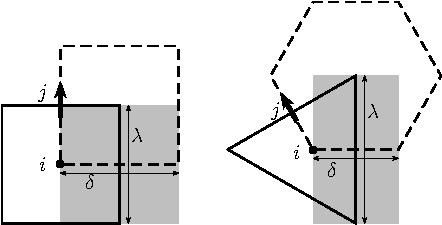
\includegraphics{fig_primal_dual.pdf}
\end{center}
\caption{Pairs of primal (solid line borders) and dual (dashed line borders) grids for quadrilateral and triangular primal meshes -- horizontal projection of grid cell volumes. Further explanations are given in the text.}
\label{grid}
\end{figure}

\subsection{Discrete operators}

First, we have to specify the spatial operators on the grid. We can interpret the grid as an arrangement of two grid types, a primal and a dual grid (Bonaventura and Ringler, 2005), which is shown in Figure \ref{grid} for a pair of
quadrilateral meshes and a pair of triangular and hexagonal grids. For the ICON model, the triangular grid is referred to as
the primal grid, but the opposite choice is also possible (Thuburn 2008, Thuburn et al. 2009, Torsvik et al.~2005), and implemented as in option in ICON.  
Each edge of
a primal cell is orthogonal to one edge of a dual cell. We use here a horizontal C-grid arrangement, for which the normal wind component locations $n$ are defined at the centers of the primal grid edges (faces in three dimensions) and point normal to them. Their direction is thought of as pointing outwards with respect to the primal cell center $i$. The scalar quantities
are to be found at the cell centers $i$.
In three dimensions, we combine a horizontal C-grid with a vertical L-grid. Then, the vorticity components are placed at the edge centers of the primal grid box and point tangential to this edge.

The generalized Gauss theorem is invoked for evaluating the vorticity components on the grid
\begin{equation}
 \int_V\nabla \times \mathbf{v} d\tau =-\oint_S \mathbf{v}\times d\mathbf{s}.
\end{equation}
The RHS of this equation is discretely represented by a sum over the faces of a dual grid box. The divergence operator is similarly defined via the Gauss theorem
\begin{equation}
 \int_V\nabla \cdot \mathbf{g} d\tau =\oint_S \mathbf{g} \cdot d\mathbf{s},
\end{equation}
where $\mathbf{g}$ is an arbitrary flux. The discretized version ends up in a sum over the faces of a primal grid box for the RHS that uses contravariant base vectors for the surface elements and covariant ones for the fluxes\footnote{Refer to
Bonavetura and Ringler (2005) for details on the use of integral theorems for the discretisation in the ICON model.}.

\subsection{Spatial discretisation of the brackets}

For the discretisation of the Poisson and Nambu brackets, the divergence and the rotation operators are the only ones needed.
In particular, the gradient operator follows as the dual counterpart of the divergence operator. This duality is connected with the foundation on which the two previously introduced Poisson brackets are built, namely the rule of integration by parts. That rule is also the background of the Arakawa Jacobian (cf.~Salmon and Talley, 1989; and Salmon, 2007). The discretised form of the mass bracket reads
\begin{align}
& \{\mathcal{F},\mathcal{H}\}_{\varrho}\Rightarrow\label{massbracket}\\
&-\sum_{m=1}^M\left[
\frac{\delta\mathcal{F}}{\delta\varrho}\Big|_m\left(\nabla\cdot\frac{\delta\mathcal{H}}{\delta\mathbf{v}}\right)_m
-\frac{\delta\mathcal{H}}{\delta\varrho}\Big|_m\left(\nabla\cdot\frac{\delta\mathcal{F}}{\delta\mathbf{v}}\right)_m
\right]V_m\nonumber\\
&=-\sum_{m=1}^M\left[
\frac{\delta\mathcal{F}}{\delta\varrho}\Big|_m\left(\nabla\cdot\frac{\delta\mathcal{H}}{\delta\mathbf{v}}\right)_m
+\left(\frac{\delta\mathcal{F}}{\delta\mathbf{v}}\cdot\nabla\frac{\delta\mathcal{H}}{\delta\varrho}\right)_m
\right]V_m,\nonumber
\end{align}
where the boundary conditions as in the analytical case are tacitly taken into account.
Consequently, the divergence and the gradient operators obey a discrete version of
\begin{equation}
 \int_V \psi \nabla\cdot \mathbf{g} d\tau = -\int_V \mathbf{g}\cdot\nabla\psi d\tau
\end{equation}
for arbitrary vector fluxes $\mathbf{g}$ and scalars $\psi$. The consequence for the model designer is that the divergence operator defines already the gradient operator. There is no direct reference to the gradient operator. It will be created automatically when writing down the equations for the prognostic variables for which $\delta\mathcal{F}/\delta\mathbf{v}$
does not vanish.

We assumed so far, that the functional derivatives $\delta\mathcal{H}/\delta\varrho$ are located in the center $i$ of the primal grid box and that those of $\delta\mathcal{H}/\delta\mathbf{v}$ are defined as normal vector
components at the faces $j$. But we have not yet defined the Hamiltonian on the grid, so that our assumptions
are initially speculative.
For the evaluation of the Hamiltonian, especially its kinetic energy part, we need
the definition of an inner product at
the center point of the primal grid. This is obtained by inspecting the role of the inner product in $\nabla\cdot\nabla\psi=\triangle\psi$. Illustratively and with direct reference to Figure \ref{grid}, we restrict ourselves again to a plane and find
\begin{equation}
\nabla\cdot\nabla\psi|_i=\frac{1}{A_i}\sum_{j\in i}\lambda_j \frac{(\psi_{o}-\psi_{i})_n}{\delta_j}
=\frac{1}{A_j}\sum_{j\in i}\frac{1}{\delta_j/2}\;\frac{(\psi_{o}-\psi_{i})_j}{\delta_j}\;\frac{\lambda_j\delta_j}{2},
\end{equation}
where $A_i$ is the area of the primal grid surrounded by the edges $j$,
$\lambda_j$ and $\delta_j$ are the lengths of the primal edges and the dual edges, respectively. The $\psi_o$ values refer to the
outer (neighbouring) $\psi$ values. Thus, the sought-for inner product on a plane is
\begin{equation}
 \mathbf{A}\cdot\mathbf{B}|_i=\frac{1}{A_i}\sum_{j\in i}a_jb_j \frac{A_{e,j}}{2},
\end{equation}
where $A_{e,j}=\delta_j\lambda_j$ is refered to as the elemental area (the grey area in Figure \ref{grid}), and $a_j$ and $b_j$ are the nomal components of the vectors at the
edges. Similar considerations hold for three dimensional volume boxes $V_i$ and elemental volumes $V_{e,j}$, where one could easily include terrain following coordinates.
